\documentclass{beamer}
\usepackage[utf8]{inputenc}

\usetheme{Madrid}
\usecolortheme{default}
\usepackage{amsmath,amssymb,amsfonts,amsthm}
\usepackage{txfonts}
\usepackage{tkz-euclide}
\usepackage{listings}
\usepackage{adjustbox}
\usepackage{array}
\usepackage{tabularx}
\usepackage{gvv}
\usepackage{lmodern}
\usepackage{circuitikz}
\usepackage{tikz}
\usepackage{graphicx}

\setbeamertemplate{page number in head/foot}[totalframenumber]

\usepackage{tcolorbox}
\tcbuselibrary{minted,breakable,xparse,skins}



\definecolor{bg}{gray}{0.95}
\DeclareTCBListing{mintedbox}{O{}m!O{}}{%
	breakable=true,
	listing engine=minted,
	listing only,
	minted language=#2,
	minted style=default,
	minted options={%
		linenos,
		gobble=0,
		breaklines=true,
		breakafter=,,
		fontsize=\small,
		numbersep=8pt,
		#1},
	boxsep=0pt,
	left skip=0pt,
	right skip=0pt,
	left=25pt,
	right=0pt,
	top=3pt,
	bottom=3pt,
	arc=5pt,
	leftrule=0pt,
	rightrule=0pt,
	bottomrule=2pt,
	toprule=2pt,
	colback=bg,
	colframe=orange!70,
	enhanced,
	overlay={%
		\begin{tcbclipinterior}
			\fill[orange!20!white] (frame.south west) rectangle ([xshift=20pt]frame.north west);
	\end{tcbclipinterior}},
	#3,
}
\lstset{
	language=C,
	basicstyle=\ttfamily\small,
	keywordstyle=\color{blue},
	stringstyle=\color{orange},
	commentstyle=\color{green!60!black},
	numbers=left,
	numberstyle=\tiny\color{gray},
	breaklines=true,
	showstringspaces=false,
}
%------------------------------------------------------------
%This block of code defines the information to appear in the
%Title page
\title %optional
{2.10.70}

%\subtitle{A short story}

\author % (optional)
{Nipun Dasari - EE25BTECH11042}



\begin{document}
	
	
	\frame{\titlepage}
	\begin{frame}{Question}
		In a $\triangle \text{ABC}$, D and E are points on $BC$ and $AC$ respectively, such that $BD = 2DC$ and $AE = 3EC$. Let P be the point of intersection of $AD$ and $BE$. Find $\frac{BP}{PE}$ using vector methods. 
	\end{frame}

		
	\begin{frame}{Theoretical Solution}
			Let vertex A be the origin. The position vectors are:
		\begin{align}
			\vec{a} = \vec{0}, \quad \vec{b} = \text{Position vector of B}, \quad \vec{c} = \text{Position vector of C}
		\end{align}
		
		Position vector of point D, which divides BC in the ratio $2:1$:
		\begin{align}
			\vec{d} = \frac{1\vec{b} + 2\vec{c}}{2+1} = \frac{\vec{b} + 2\vec{c}}{3}
		\end{align}
		Position vector of point E, which divides AC in the ratio $3:1$:
		\begin{align}
			\vec{e} = \frac{1\vec{a} + 3\vec{c}}{3+1} = \frac{3\vec{c}}{4}
		\end{align}
		
		Let P divide AD in the ratio $AP:PD = \lambda:1$. The position vector of P is:
	\end{frame}
	\begin{frame}{Theoretical Solution}
		\begin{align}
			\vec{p} = \frac{1\vec{a} + \lambda\vec{d}}{\lambda+1} = \frac{\lambda}{\lambda+1} \vec{d}
		\end{align}
		Substituting for $\vec{d}$:
		\begin{align}
			\vec{p} = \brak{ \frac{\lambda}{\lambda+1} } \brak{ \frac{\vec{b} + 2\vec{c}}{3} } = \frac{\lambda}{3\brak{\lambda+1}}\vec{b} + \frac{2\lambda}{3\brak{\lambda+1}}\vec{c} \label{eq:1}
		\end{align}
		
		Let P divide BE in the ratio $BP:PE = \mu:1$. The position vector of P is:
		\begin{align}
			\vec{p} = \frac{1\vec{b} + \mu\vec{e}}{\mu+1}
		\end{align}
		Substituting for $\vec{e}$:
	\end{frame}
	\begin{frame}{Theoretical Solution}
		\begin{align}
			\vec{p} = \frac{1}{\mu+1}\vec{b} + \frac{\mu}{\mu+1} \vec{e} = \frac{1}{\mu+1}\vec{b} + \frac{\mu}{\mu+1} \brak{ \frac{3\vec{c}}{4} } = \frac{1}{\mu+1}\vec{b} + \frac{3\mu}{4\brak{\mu+1}}\vec{c} \label{eq:2}
		\end{align}
		
		Since $\vec{b}$ and $\vec{c}$ are non-collinear, we equate their coefficients from \eqref{eq:1} and \eqref{eq:2}.\\
		Coefficients of $\vec{b}$:
		\begin{align}
			\frac{\lambda}{3\brak{\lambda+1}} = \frac{1}{\mu+1} \label{eq:3}
		\end{align}
		Coefficients of $\vec{c}$:
		\begin{align}
			\frac{2\lambda}{3\brak{\lambda+1}} = \frac{3\mu}{4\brak{\mu+1}} \label{eq:4}
		\end{align}
	\end{frame}
	\begin{frame}{Theoretical Solution}
		From \eqref{eq:3} and \eqref{eq:4}, we can see that the LHS of \eqref{eq:4} is twice the LHS of \eqref{eq:3}.
		\begin{align}
			2 \brak{\frac{1}{\mu+1}} = \frac{3\mu}{4\brak{\mu+1}}
		\end{align}
		Multiplying both sides by $4\brak{\mu+1}$:
		\begin{align}
			8 = 3\mu \implies \mu = \frac{8}{3}
		\end{align}
		The required ratio is $BP:PE = \mu:1$.
		\begin{align}
			\therefore	\frac{BP}{PE} = \mu = \frac{8}{3}
		\end{align}
	\end{frame}
	
	\begin{frame}[fragile]
		\frametitle{C Code -  formula function }
		
		\begin{lstlisting}
		void calculate_points_from_arrays(
		double* input_A,      // Pointer to a 2-element array [Ax, Ay]
		double* input_B,      // Pointer to a 2-element array [Bx, By]
		double* input_C,      // Pointer to a 2-element array [Cx, Cy]
		double* output_points // Pointer to a 12-element array to be filled
		) {
			// Unpack input points for clarity
			double Ax = input_A[0], Ay = input_A[1];
			double Bx = input_B[0], By = input_B[1];
			double Cx = input_C[0], Cy = input_C[1];
		\end{lstlisting}
	\end{frame}
	\begin{frame}[fragile]
		\frametitle{C Code -  formula function }
		
		\begin{lstlisting}
		 // Calculate Point D
		double Dx = (1.0 * Bx + 2.0 * Cx) / 3.0;
		double Dy = (1.0 * By + 2.0 * Cy) / 3.0;
		
		// Calculate Point E
		double Ex = (1.0 * Ax + 3.0 * Cx) / 4.0;
		double Ey = (1.0 * Ay + 3.0 * Cy) / 4.0;
		
		// Calculate Point P
		double mu = 8.0 / 11.0;
		double Px = (1.0 - mu) * Bx + mu * Ex;
		double Py = (1.0 - mu) * By + mu * Ey;
			\end{lstlisting}
		\end{frame}
	\frametitle{C Code -  formula function }
	\begin{frame}[fragile]
		\frametitle{C Code -  formula function }
	\begin{lstlisting}
	// Fill the output array (12 elements: Ax, Ay, Bx, By, ...)
	output_points[0] = Ax; output_points[1] = Ay;
	output_points[2] = Bx; output_points[3] = By;
	output_points[4] = Cx; output_points[5] = Cy;
	output_points[6] = Dx; output_points[7] = Dy;
	output_points[8] = Ex; output_points[9] = Ey;
	output_points[10] = Px; output_points[11] = Py;
	}
	\end{lstlisting}
	\end{frame}
	
	\begin{frame}[fragile]
		\frametitle{Python Code through shared output}
		\begin{lstlisting}
	import ctypes
	import numpy as np
	import matplotlib.pyplot as plt
	
	# --- Step 1: Load the shared library ---
	lib = ctypes.CDLL('./2.10.70.so')
	
	# --- Step 2: Define the C function signature using NumPy-aware pointers ---
	calculate_points = lib.calculate_points_from_arrays
	
	# Define the argument types. 'ndpointer' creates a ctypes-compatible type for NumPy arrays.
	calculate_points.argtypes = [
	np.ctypeslib.ndpointer(dtype=np.double, ndim=1, flags='C_CONTIGUOUS'), # input_A
	np.ctypeslib.ndpointer(dtype=np.double, ndim=1, flags='C_CONTIGUOUS'), # input_B
	np.ctypeslib.ndpointer(dtype=np.double, ndim=1, flags='C_CONTIGUOUS'), # input_C
	np.ctypeslib.ndpointer(dtype=np.double, ndim=1, flags='C_CONTIGUOUS')  # output_points
	]
		\end{lstlisting}
	\end{frame}
	
	\begin{frame}[fragile]
		\frametitle{Python Code through shared output}
		\begin{lstlisting}
	# The function has a 'void' return type in C
	calculate_points.restype = None
	
	# --- Step 3: Prepare NumPy arrays and call the C function ---
	# Define the vertices of the triangle as NumPy arrays
	A = np.array([0.0, 0.0], dtype=np.double)
	B = np.array([6.0, 1.0], dtype=np.double)
	C = np.array([2.0, 5.0], dtype=np.double)
	
	# Create an empty NumPy array for the C function to fill
	# It needs to have space for 6 points (6 * 2 = 12 doubles)
	output_data = np.zeros(12, dtype=np.double)
	
	# Call the C function. NumPy arrays are passed directly.
	calculate_points(A, B, C, output_data)
	
		\end{lstlisting}
	\end{frame}
	\begin{frame}[fragile]
		\frametitle{Python Code through shared output}
		\begin{lstlisting}
	# --- Step 4: Reshape the output and plot ---
	# Reshape the flat output array into a 6x2 array (6 points, 2 coords each)
	points_array = output_data.reshape(6, 2)
	
	point_names = ['A', 'B', 'C', 'D', 'E', 'P']
	points = {name: coord for name, coord in zip(point_names, points_array)}
	
	print("Coordinates calculated by C library and loaded into NumPy:")
	for name, coords in points.items():
	print(f"  Point {name}: ({coords[0]:.4f}, {coords[1]:.4f})")
	
	# Plotting logic remains the same
	fig, ax = plt.subplots(figsize=(10, 8))
	ax.set_aspect('equal', adjustable='box')
	ax.grid(True, linestyle=':', alpha=0.7)
	
	triangle = plt.Polygon(points_array[:3], edgecolor='darkblue', facecolor='lightblue', alpha=0.4, linewidth=2, label='Triangle ABC')
	ax.add_patch(triangle)
	
		\end{lstlisting}	
	\end{frame}
		\begin{frame}[fragile]
		\frametitle{Python Code through shared output}
		\begin{lstlisting}
			for name, coords in points.items():
			color = 'red' if name == 'P' else 'black'
			size = 12 if name == 'P' else 8
			ax.plot(coords[0], coords[1], 'o', markersize=size, color=color, label=f'Point {name}')
			ax.text(coords[0] + 0.15, coords[1] + 0.15, name, fontsize=14, fontweight='bold', color=color)
			
			ax.set_title('Plot from C Library using NumPy and ctypes', fontsize=16)
			ax.legend(loc="upper left")
			
			plt.figure()
			plt.savefig('numpy_ctypes_plot.png')
			
			plt.show()
			
		\end{lstlisting}	
	\end{frame}
	
	\begin{frame}[fragile]
		\frametitle{Python code : Direct }
		
		\begin{lstlisting}
			import numpy as np
			import matplotlib.pyplot as plt
			
			def solve_and_plot_with_numpy():
			"""
			Calculates and plots the triangle intersection using NumPy.
			"""
			# --- Step 1: Define vertices as NumPy arrays ---
			# We choose A as the origin, consistent with the vector solution.
			A = np.array([0.0, 0.0])
			B = np.array([6.0, 1.0])
			C = np.array([2.0, 5.0])
			
			# --- Step 2: Calculate points D and E using vector arithmetic ---
			# Point D on BC such that BD:DC = 2:1
			# Vector formula: D = (1*B + 2*C) / 3
			D = (1 * B + 2 * C) / 3
		\end{lstlisting}
	\end{frame}
	\begin{frame}[fragile]
		\frametitle{Python code : Direct }
		
		\begin{lstlisting}
		 # --- Step 3: Calculate the intersection point P ---
		# From the vector solution, we found the ratio mu for the line BE is 8/11.
		# Vector formula: P = (1-mu)*B + mu*E
		mu = 8.0 / 11.0
		P = (1 - mu) * B + mu * E
		
		# --- Step 4: Plot the results ---
		points = {'A': A, 'B': B, 'C': C, 'D': D, 'E': E, 'P': P}
		
		print("Coordinates calculated by NumPy:")
		for name, coords in points.items():
		print(f"  Point {name}: ({coords[0]:.4f}, {coords[1]:.4f})")
		
		# Setup plot
		fig, ax = plt.subplots(figsize=(10, 8))
		ax.set_aspect('equal', adjustable='box')
		ax.grid(True, linestyle=':', alpha=0.7)
		
		# Plot triangle, lines, and points
		triangle = plt.Polygon([A, B, C], edgecolor='darkblue', facecolor='lightblue', alpha=0.4, linewidth=2, label='Triangle ABC')
		ax.add_patch(triangle)
		\end{lstlisting}
	\end{frame}
	\begin{frame}[fragile]
		\frametitle{Python code : Direct }
		
		\begin{lstlisting}
		ax.plot([A[0], D[0]], [A[1], D[1]], 'r--', label='Line AD')
		ax.plot([B[0], E[0]], [B[1], E[1]], 'g--', label='Line BE')
		
		for name, coords in points.items():
		color = 'red' if name == 'P' else 'black'
		size = 12 if name == 'P' else 8
		ax.plot(coords[0], coords[1], 'o', markersize=size, color=color, label=f'Point {name}')
		ax.text(coords[0] + 0.15, coords[1] + 0.15, name, fontsize=14, fontweight='bold', color=color)
		
		ax.set_title('Geometric Solution using Python and NumPy', fontsize=16)
		ax.set_xlabel('X-axis', fontsize=12)
		ax.set_ylabel('Y-axis', fontsize=12)
		ax.legend(loc="upper left")
		
		plt.savefig('numpy_plot.png')
		
		plt.show()
		\end{lstlisting}
	\end{frame}
	
	
	\begin{frame}{Plot by python using shared output from c}
		\begin{figure}[H]
			\centering
			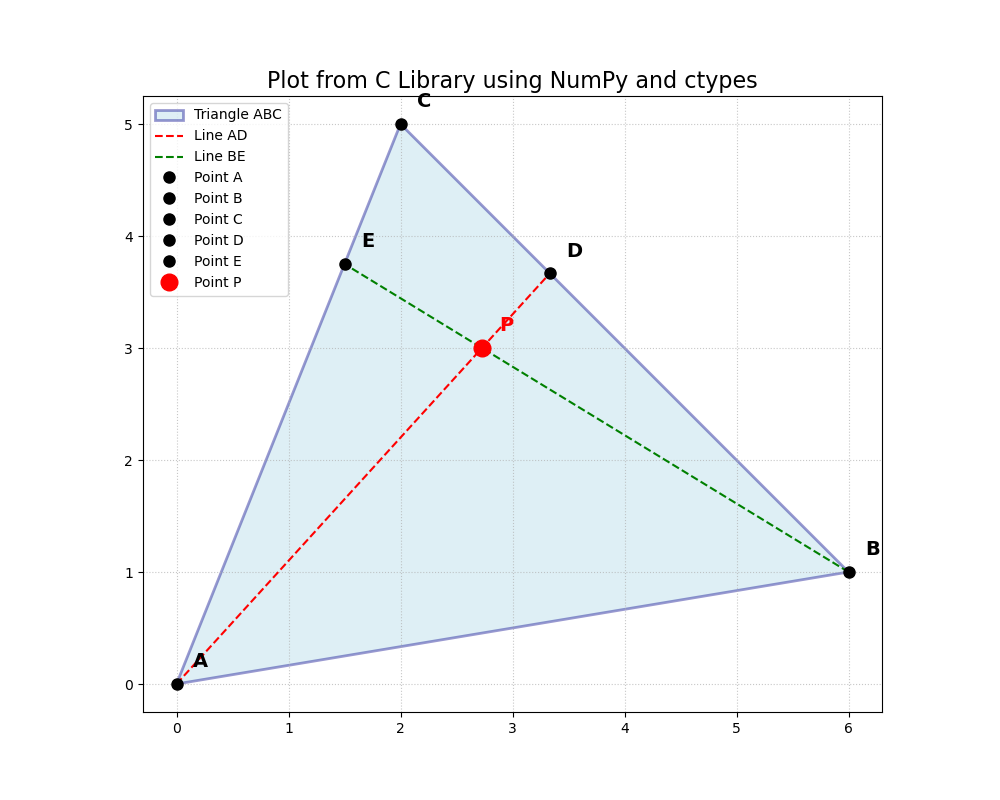
\includegraphics[width = 0.6\columnwidth]{figs/Figure_1.png}
			\caption*{}
			\label{fig1}
		\end{figure}
	\end{frame}
	
	\begin{frame}{Plot by python only}
		\begin{figure}[H]
			\centering
			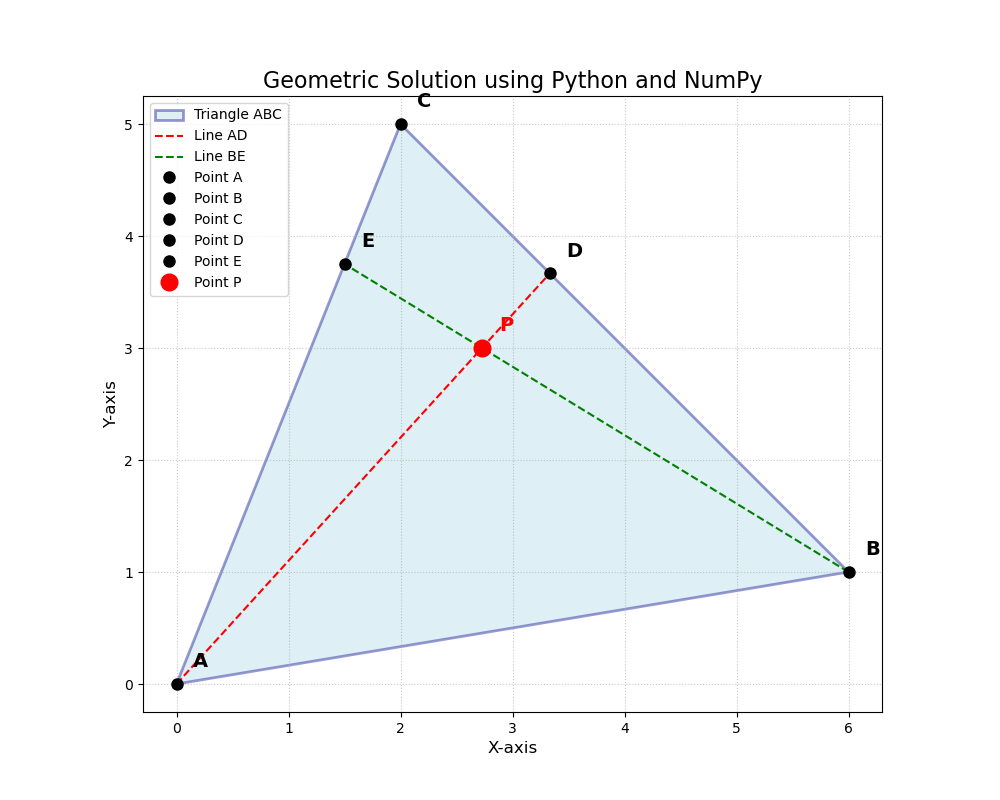
\includegraphics[width = 0.6\columnwidth]{figs/Figure_2.png}
			\caption*{}
			\label{fig2}
		\end{figure}
	\end{frame}
	
	
	
\end{document}